\section{Theorie}
\label{sec:Theorie}

\subsection{Einleitung}
Ziel dieses Versuches ist es, die Eigenschaften eines RLC-Schwingkreises
zu bestimmen. Dafür werden Messungen mit Variation des Widerstandes oder der
Frequenz durchgeführt.

\subsection{Theoretische Grundlagen}
Ein RLC-Kreis stellt einen gedämpften Schwingkreis dar. Die Schwingung besteht
aus einer Verschiebung der elektromagnetischen Energie zwischen
Spule (L) und Kondensator (C).
Dabei ändert der Strom periodisch sein
Vorzeichen.
\begin{figure}
  \centering
  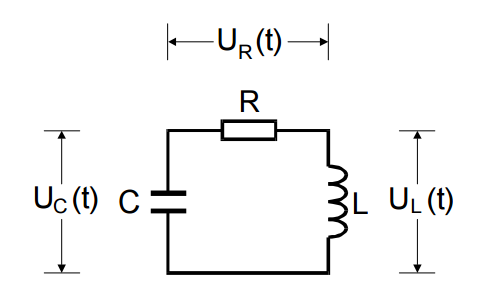
\includegraphics{schwingkreis.png}
  \caption{Gedämpfter Schwingkreis}
  \label{fig:RLC}
\end{figure}
Eine schematische Darstellung ist in \ref{fig:RLC} zu sehen.
Die Differentialgleichung eines RLC-Kreises entspricht der eines harmonischen
Oszillators:
\begin{equation}
   \frac{d^2I}{dt^2} + \frac{R}{L} \frac{dI}{dt} + \frac{I}{LC} = 0.
   \label{eqn:dgl}
\end{equation}
Entsprechen ergeben sich die Lösungen zu:
\begin{equation}
  I(t) = I_1 e^{j\omega_1t} + I_2 e^{j\omega_2t}
  \label{eqn:I}
\end{equation}
  mit
\begin{equation}
  \omega_{1,2} = j\frac{R}{2L} \pm \sqrt{\frac{1}{LC} - \frac{R^2}{4L^2}}.
  \label{eqn:omega}
\end{equation}
Dabei ist j die imaginäre Einheit.
Wie unschwer an Gleichung \ref{eqn:omega} zu erkennen ist müssen abhängig von
den Parametern R, L und C nun 3 Fälle unterschieden werden.

\subsubsection{Fall 1: $\frac{1}{LC} <= \frac{R^2}{4L^2}$}

In dem Fall $\frac{1}{LC}<\frac{R^2}{4L^2}$ ist der Ausdruck in der
Wurzel imaginär, in Gleichung
\ref{eqn:I} kommen also nur noch reelle Exponentialfunktionen vor. Diese
beschreiben allerdings keine Schwingung, sondern die
\textbf{aperiodische Dämpfung}. Nach einer gewissen Zeitspanne liegt dabei ein
gewöhnliches Relaxationsverhalten vor, vorher kann allerdings noch ein Extremwert
durchschritten werden.
Den Fall $\frac{1}{LC}=\frac{R^2}{4L^2}$ bezeichnet man als
\textbf{aperiodischen Grenzfall}. Der Wurzelterm in Gleichung \ref{eqn:omega}
verschwindet und I(t) geht schnellstmöglichst gegen null.
Beide Fälle sind in Abb.\ref{fig:aper} dargestellt, die gestrichelte Linie zeigt
den aperiodischen Grenzfall, die anderen mögliche Verläufe einer aperiodischen
Dämpfung:
\begin{figure}
  \centering
  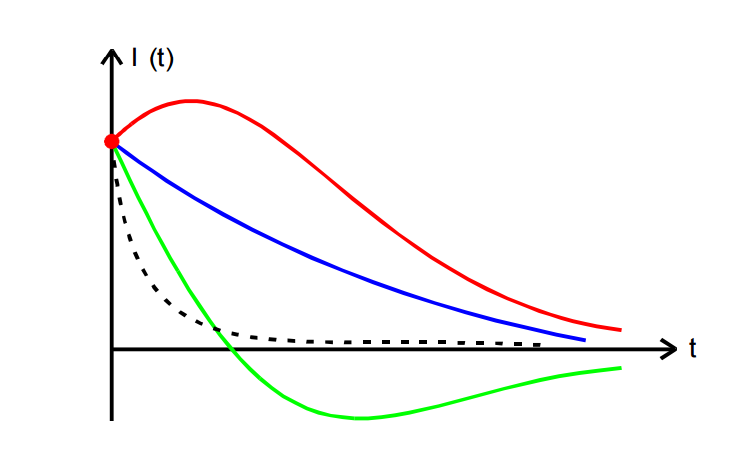
\includegraphics{aperiode.png}
  \caption{Stromverlauf in einem aperiodisch gedämpften System}
  \label{fig:aper}
\end{figure}

\subsubsection{Fall 2: $\frac{1}{LC}>\frac{R^2}{4L^2}$}
Unter dieser Bedingung ist der Term unter der Wurzel in Gleichung
\ref{eqn:omega} positiv,
die Wurzel also reell. Damit muss $I_1 = I_2$ sein und für den Strom ergibt
sich:
\begin{equation}
  I(t) = A_0e^{-2\pi \mu t}\cos{(2\pi \nu t + \eta)}.
  \label{eqn:Ischwingung}
\end{equation}
Dabei beschreibt die einhüllende $e$-Funktion die Dämpfung und der
Kosinus-Term die Schwingungseigenschaft des Systems. $\nu$ entspricht der
Frequenz.
2 wichtige Eigenschaften des Schwingkreises bestehen in der Schwingungsdauer
\begin{equation}
  T =\frac{1}{\nu} = \frac{2\pi}{\sqrt{1/LC - R^2/4L^2}}
\end{equation}
und der Abklingdauer
\begin{equation}
  T_{ex} = \frac{1}{2\pi\mu} = \frac{2L}{R}.
\end{equation}
Als Abklingdauer wird die Zeit bezeichnet, nach der die Amplitude auf den e-ten
Teil ihres ursprünglichen Wertes abgefallen ist.

\begin{figure}
  \centering
  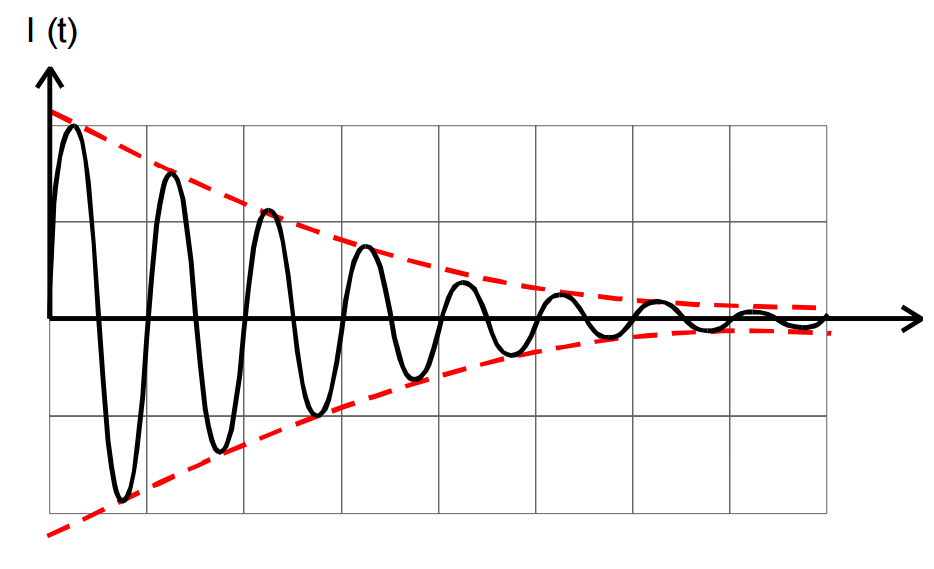
\includegraphics[width=\textwidth]{gedschwingung.png}
  \caption{Spannungsverlauf bei einer gedämpften Schwingung}
  \label{fig:gedschw}
\end{figure}
Ein solches gedämpftes Schwingungsverhalten ist in \ref{fig:gedschw} dargestellt.
Die Lösung für den ungedämpften Schwingkreis erhält man über den selben Weg mit
der Annahme, dass $\frac{1}{LC} >> \frac{R^2}{4L^2}$ sei.

\subsubsection{Angeregter Schwingkreis}
Für eine erzwungene Schwingung wird der Schwingkreis von einer äußeren
sinusförmigen
Wechselspannung kontinuierlich angetrieben.
Die komplexe DGL wird also inhomogen und sieht wie folgt aus:
\begin{equation}
  \centering
  \frac{d^2I}{dt^2} + \frac{R}{L} \frac{dI}{dt}
  + \frac{I}{LC} = U_0\exp{j\omega t}
  \label{eqn:Iinh}
\end{equation}
Wie zuvor entspricht j der imaginären Enheit, die rechte Seite der Gleichung
stellt die anregende Spannung dar.
Abhängig von der Frequenz dieser
Spannungsquelle variieren Spannungsamplitude und Phasenverschiebung zwischen
Generator und Kondensator:
\begin{equation}
  \phi(\omega) = \arctan{\frac{-\omega R C}{1 - LC\omega^2}}
  \label{eqn:phi}
\end{equation}
\begin{equation}
  U_c(\omega) = \frac{U_0}{\sqrt{(1 - LC\omega^2)^2 + \omega^2R^2C^2}}
  \label{eqn:Uc}
\end{equation}
Dabei bezeichnet $\phi$ die Phasenverschiebung und $U_c$ die Spannung am
Kondensator.
Von besonderer Bedeutung ist die Resonanzfrequenz $\omega_{res}$, bei der
$U_c$ ein Maximum erreicht, das größer ist als $U_0$:
\begin{equation}
  \omega_{res} = \sqrt{\frac{1}{LC} - \frac{R^2}{2L^2}}.
  \label{eqn:wres}
\end{equation}
Außerdem erkennt man an \ref{eqn:Uc}, dass $U_c$ für
$\omega \rightarrow \infty$ gegen 0 und für $\omega \rightarrow 0$ gegen $U_0$
geht.
Eine weitere charakteristische Größe eines angeregten Schwingkreises ist die
Güte oder Resonanzüberhöhung, gegeben durch:
\begin{equation}
  U_{Cmax} = \frac{1}{\omega_0 R C} \cdot U_0 = \frac{1}{R}\sqrt{\frac{L}{C}}U_0.
  \label{eqn:güte1}
\end{equation}
Die Größe $\frac{1}{\omega_0 R C}$ entspricht dabei der Güte $q$ des Schwingkreises.
Außerdem lässt sich zwischen Güte und Schärfe der Resonanz folgender
Zusammenhang herstellen:
\begin{equation}
  q = \frac{\omega_0}{\omega_+ - \omega_-}.
  \label{eqn:güte2}
\end{equation}
Dabei bezeichnen $\omega_-$ und $\omega_+$ die Frequenzen bei denen $U_c$ dem
1/$\sqrt{2}$ -fachen des Maximums entspricht.
